%%%%%%%%%%%%%%%%%%%%%%%%%%%%%%%%%%%%%%%%%%%%
% Introduction
%%%%%%%%%%%%%%%%%%%%%%%%%%%%%%%%%%%%%%%%%%%%




\chapter{Introduction}

\begin{figure}
\center
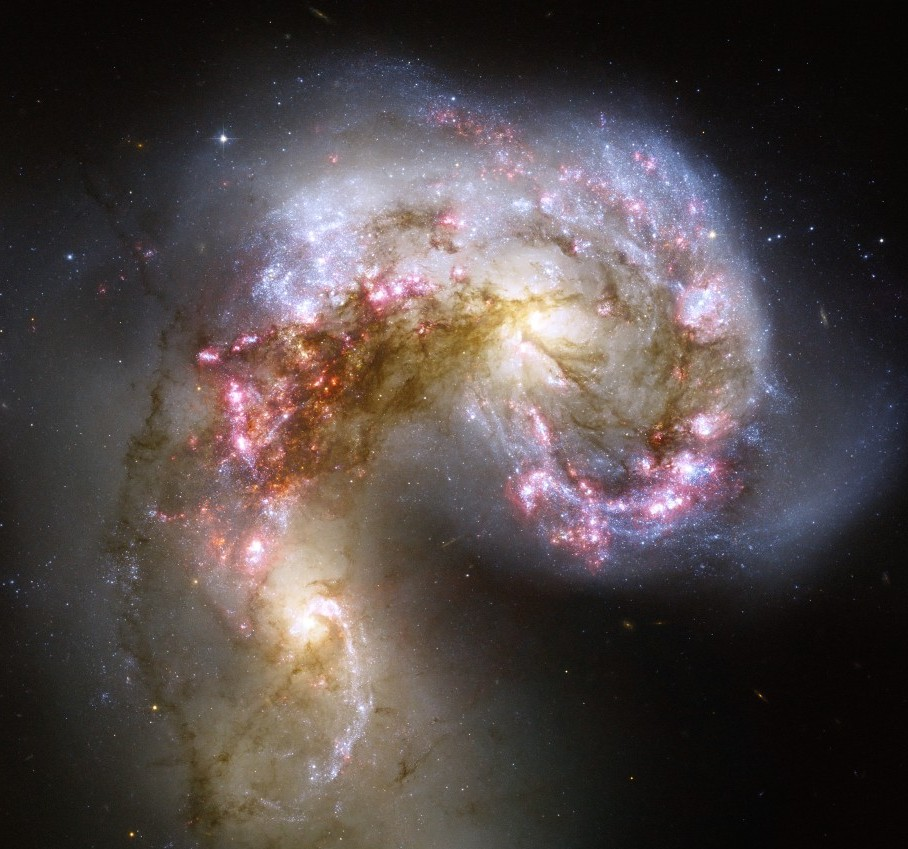
\includegraphics[width=0.7\linewidth]{Figures/0_antennas.jpg}
\caption{Composite picture (visible and infrared) of the merging Antennaes galaxies (NGC 4038 and 4039). Very active star forming regions are seen in infrared as the gas is heated by newborn stars. Bright blue points are the hot OB stars found in the numerous Young Massive Clusters (\textbf{YMCs}) in the system. \textit{Credits: NASA, ESA, and B. Whitmore (STScI)}.}
\label{Fig:0_antennas}
\end{figure}

\newpage


%\section{A summary of the motivations}


Globular Clusters(\textbf{GCs}) have long been and still are considered invaluable witnesses of galaxy formation, given their old age and bond with their host galaxies. Observations of the GC specific frequency, the amount of GCs per galactic luminosity, showed elliptical galaxies harboured proportionally more globular clusters than spirals, see the review by \cite{Harris1991}. As elliptical are spiral-merger products, this pointed at merger events triggering episodes of globular cluster formations \citep{Ashman1992}.

The relation between GC populations and galaxy formation history was strengthened and made more complex by the wealth of new observations brought by the advent of the Hubble Space Telescope. First, Young Massive Clusters, considered to be young globular clusters, were found in merging galaxies such as the Antennas \citep{Whitmore1995}. Then, cluster population around galaxies were observed to be bimodal: an extended, metal-poor blue population and a more concentrated, metal-rich red population \citep{Zepf1993,Geisler1996}. These clearly had different chemical and dynamical origins. Several hypothesis have been put forward to explain this puzzling observation: some advocated for the red population being created in merger events, others put forward the collection of blue clusters through accretion of dwarf galaxies, and others defended two distinct in-situ formation events in the galaxy, see the review by \cite{Brodie2006}.


While this question remains unsettled, it is clear that understanding the formation of globular clusters is key to understand their link with the galaxy formation history. 10 years ago, a new observation brought even more complexity to our picture of cluster formation. Globular clusters had long been thought to be homogeneous single-age, single-metallicities, stellar populations. Yet, a study by \cite{Piotto2007} showed the globular cluster NGC 2808 contained at least three different stellar sequences. Many other GCs has been shown to contain multiple populations. As this cannot be explained by the natural age spread arising from a continuous star formation at the birth clusters, such observations have far-reaching implications on their formation scenario.

A possible explanation is that globular clusters formed through the merging of smaller sub-clusters. These subclusters could have different metallicities, or possibly different ages, as a chain of successive, sequentially triggered star formation events could end up in the same cluster through merging. This picture is backed up by the most recent observations of star-forming regions in the Milky Way, showing a deeply substructured Inter-Stellar Medium (\textbf{ISM}) and star formation. That massive clusters form from merging of smaller fragmented have a strong influence of their survival rate to gas expulsion and their degree of primordial mass segregation. This in turn can affect our understanding of the ties between GC formation and galactic mergers, as the mass estimates of Young Massive Clusters in the Antennas hinge on their possible primordial mass segregation \citep{McCrady2005}.

The dynamics of sub-clusters merging to form more massive systems emerged as a crucial aspect of cluster formation, and consequentially of our understanding of galaxy formation history. Hydrodynamical simulations of star cluster formation are computationally limited and can only address this issue at small scales. This work aims at circumventing this limitation through the creation of large-scale, dynamically consistent substructured initial conditions for cluster simulations, unveiling the dynamical behaviour of these massive merging systems.

\paragraph*{}
In this introduction, we first define star clusters and important dynamical concepts such as relaxation time and virial state. We then develop the current state of theory, observations and simulation on cluster formation, substructure and early dynamical evolution. Finally, we look at alternative ways to investigate substructured dynamical evolution.




\newpage

\section{What is a star cluster ?}


 What is a star cluster ? A direct, almost tautological, definition is "a group of stars". However, this includes galaxies and random line-of-sight groups. We are interested in physical objects, smaller than galaxies, in which stars are, if not bound together, at least under direct mutual gravitational influence. Such objects include open clusters, globular clusters or associations.  \cite{Lada2003} adopted the following definition: a cluster is a stellar system with N$>35$ and a density $\rho > 1~\Mo /\textrm{pc}^3$. These objects can either dissolve in less than a million year or remain bound for billions of years. In the last century, thanks to the improvement of observational technology, many  clusters have been discovered and their origins are progressively being unravelled.

Clusters are the result of bursts of star formation in Giant Molecular Clouds (\textbf{GMCs}). All stars within a cluster were born approximately at the same time, which explains the sustained interest of the community for star clusters: they are the best available stellar physics laboratories, a large population of stars sharing the same age and distance to Earth. The age of the cluster can be derived from the most massive surviving stars in the population, as stars have lifetimes inversely correlated with their masses. Overall, integrated spectral features from all members of a star cluster can provide a wealth of information. 

\begin{figure}
    \centering
    \begin{subfigure}[b]{0.55\textwidth}
        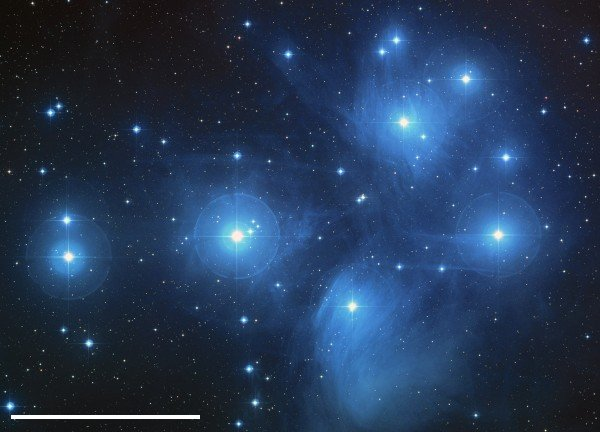
\includegraphics[width=\textwidth]{Figures/0_Pleiades_scale.jpg}
        \caption{The Pleiades, open cluster}
        \label{Fig:0_openglobular1.open}
    \end{subfigure}
    ~ 
    \begin{subfigure}[b]{0.4\textwidth}
        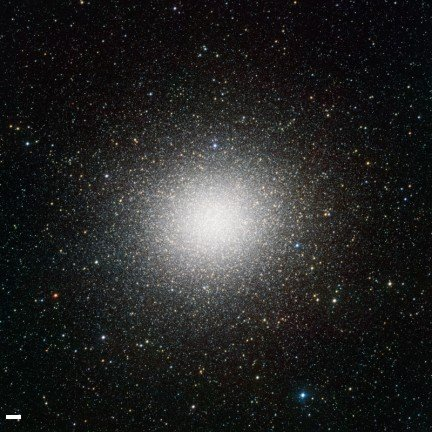
\includegraphics[width=\textwidth]{Figures/0_omega_centauri_scale.jpg}
        \caption{$\omega$ Centauri, globular cluster}
        \label{Fig:0_openglobular1.glob}
    \end{subfigure}
     \caption{Examples of various types of cluster. White bars at the lower left of each pictures show 1 parsec length scale. The dust present in the young Pleiades open cluster scatters starlight, producing this blue haze. The globular cluster $\omega$ Centauri contains one million stars and is the largest known star cluster in the Milky Way. \textit{Credits: NASA, ESA, AURA/Caltech; ESO/INAF-VST/OmegaCAM}}
     \label{Fig:0_openglobular}
\end{figure}



As we will see, clusters are also crucial to understand stellar formation. They harbour the most massive and young stars, which cause large-scale ionisation, winds and shockwaves from their explosive death in supernovaes. Massive stars caused the re-iniozation of the entire observable Universe 400 Myr after the Big Bang. To understand massive stars is to understand star formation, and to understand star formation is to understand star clusters.



%
%\begin{figure}
%\center
%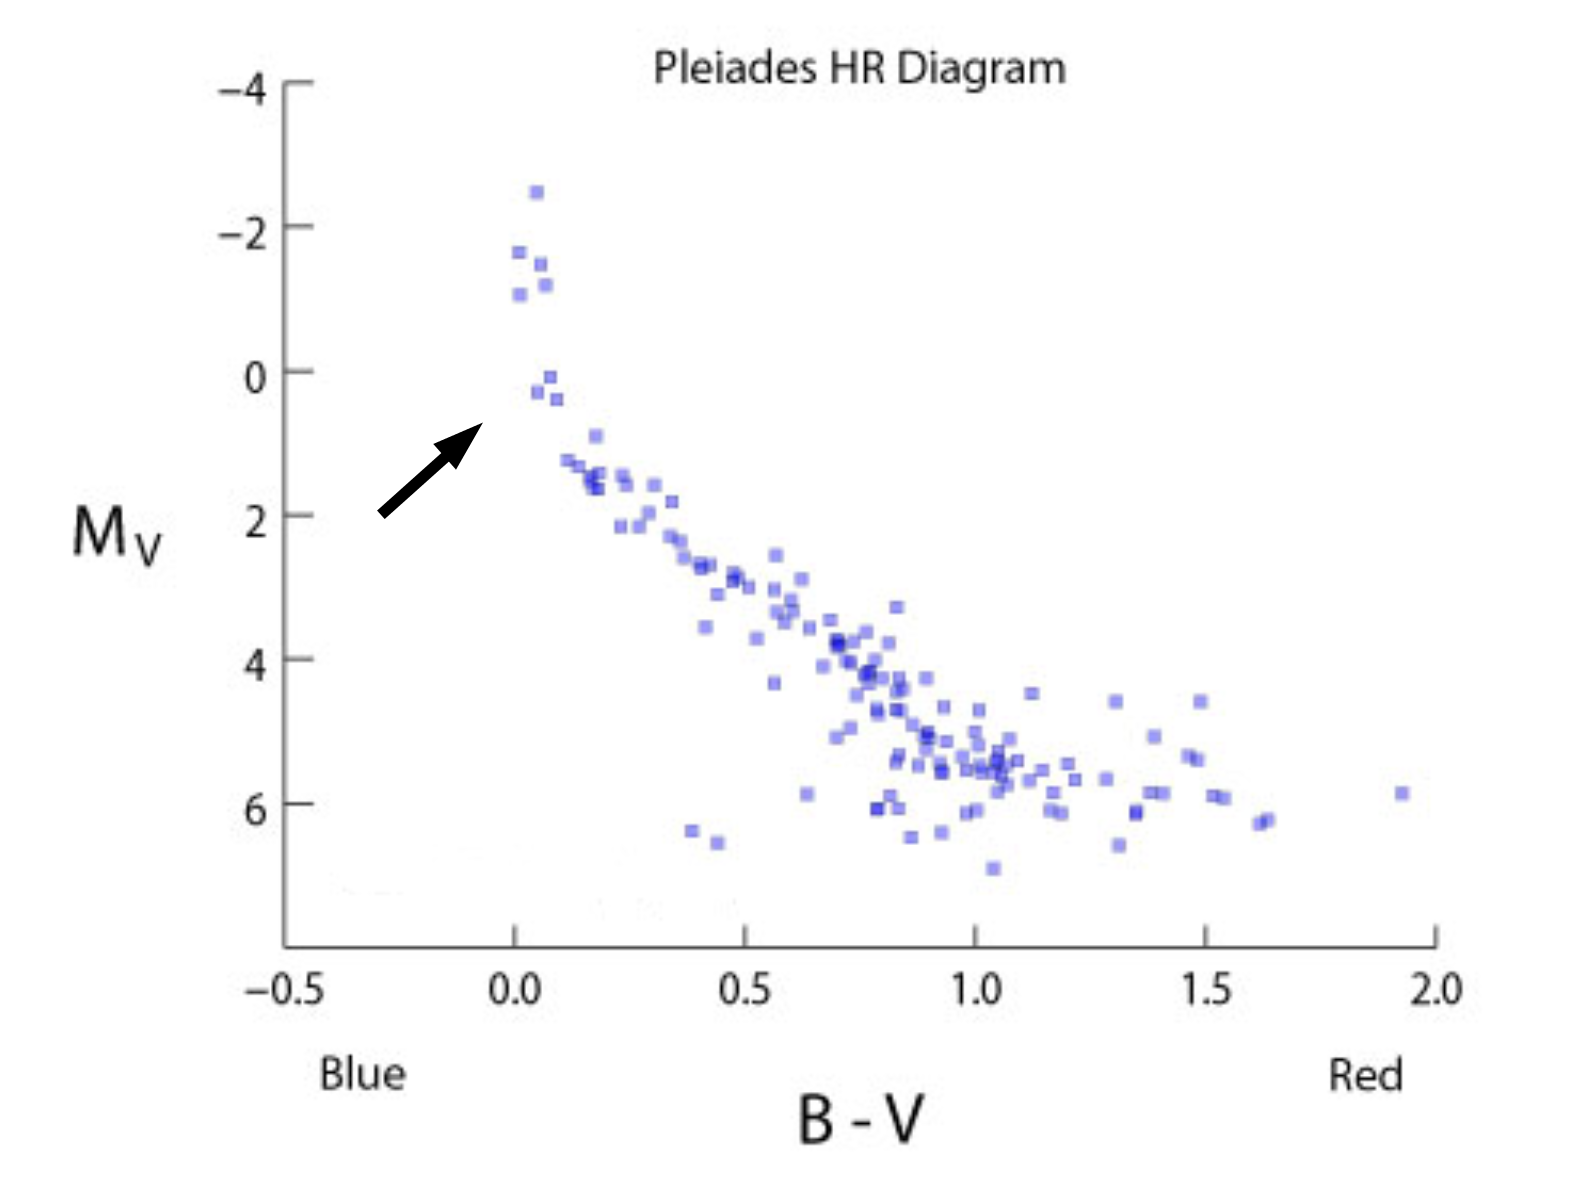
\includegraphics[width=0.45\linewidth]{Figures/0_HRDiagram_Pleiades.png}
%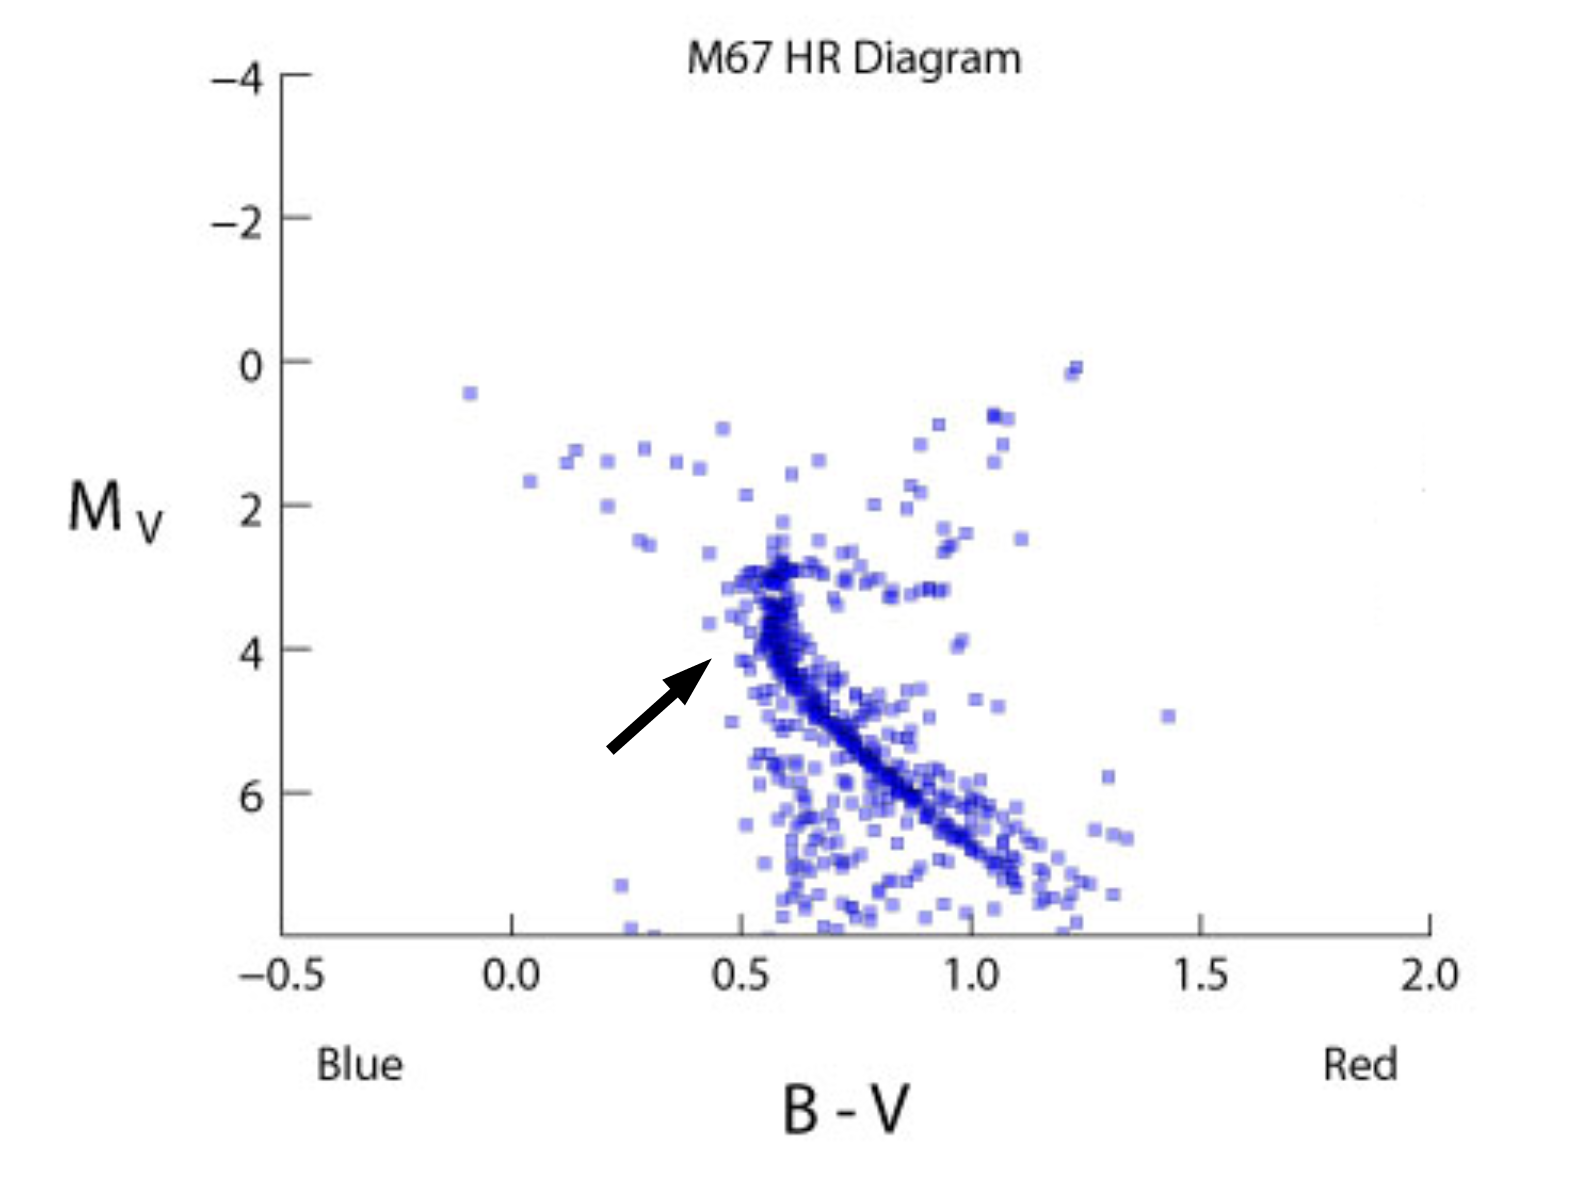
\includegraphics[width=0.45\linewidth]{Figures/0_HRDiagram_M67.png}
%\caption{Hertzprung-Russel diagram of the Pleiades and M67. An arrow points at the Main-Sequence turn-off for each cluster. The figures were taken from the \href{http://www.astrophysicsspectator.com/topics/stars/HertzsprungRussellClusters.html}{Astrophysics Spectator} website and data can be found in \protect\cite{Stassun2002,Kharchenko2004}  }
%\label{Fig:0_HR}
%\end{figure}
%
%One example is the ability to date a cluster, thus its members, through the main-sequence turn off. On figure~\ref{Fig:0_HR} is shown the Hertzprung-Russel diagram for two different clusters: The Pleiades and M67. The HR diagram shows the luminosity of the star versus its color, redder on the right, bluer on the left. Stars spend most of their life on the Main Sequence, with the most massive, luminous blue stars on the left, and red fainter smaller stars on the right. Massive stars have shorter lives and depart from the main sequence before small stars. Looking at the Main Sequence turn-off in the HR diagram of a cluster tells us the mass of the stars currently leaving the MS, which gives its age and that of all other stars. As seen on the figure, the Pleiades are younger (100Myr) than M67 ($\sim$ 4 Gyr) as the stars leaving the MS are more massive.


Star clusters are historically divided into two "classical" categories: globular clusters and open clusters. As observational technology improved, categories tended to blend into a spectrum of size, age, and dynamical state, with Young Massive Clusters, embedded clusters and OB associations. Several of these categories have significant overlap, but each one emphasizes a particular characteristic of star cluster, thus these are useful for a comprehensive discussion.


\begin{figure}
	 \begin{subfigure}[b]{0.415\textwidth}
        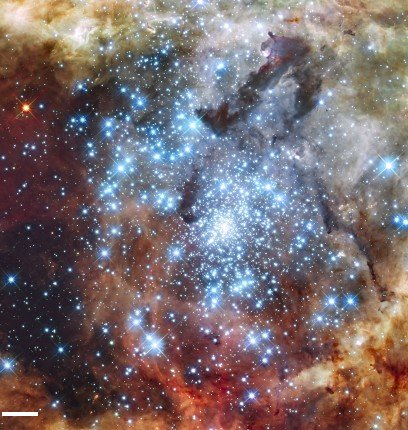
\includegraphics[width=\textwidth]{Figures/0_R136_scale.jpg}
        \caption{R136, Young Massive Cluster}
        \label{Fig:0_openglobular2.ymc}
    \end{subfigure}
    ~ 
    \begin{subfigure}[b]{0.55\textwidth}
        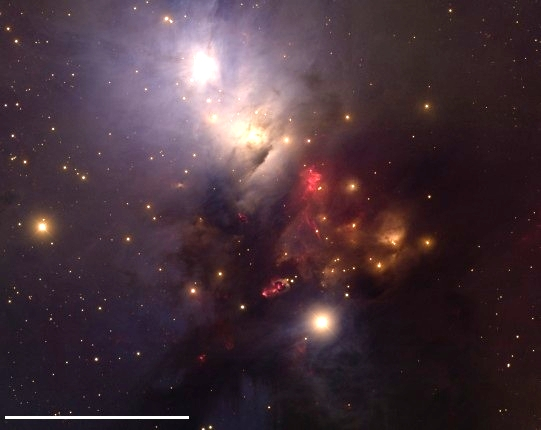
\includegraphics[width=\textwidth]{Figures/0_NGC1333_scale_contrast.jpg}
        \caption{NGC 1333, embedded cluster}
        \label{Fig:0_openglobular2.emb}
    \end{subfigure}
        \caption{Examples of various types of cluster. White bars show 1pc. The young massive cluster R136 is  surrounded by its primordial nebula while the embedded cluster NGC 1333 is still inside it. (b) is a composite of visible and infra-red light. \textit{Credits: NASA, ESA, F. Paresce;T. Rector(U.Alaska Anchorage), H. Schweiker}}
    \label{Fig:0_ymcemb}
\end{figure}

\begin{itemize}


\item[\textbf{Globular clusters}] are old and massive stellar systems, found orbiting most galaxies. Most of them are older than 10 Gyr and more massive than $10^4~M_\odot$. The most massive known Globular cluster in the Milky Way is $\omega$ Centauri, with $4~10^6~\Mo$ \citep{Dsouza2013}, see Fig~\ref{Fig:0_openglobular1.glob}. They only contain stars, without any dust or gas. The 150 known globular clusters in the Milky way are scattered in the disk and the halo, with a higher concentration near the bulge \citep{Harris1996}. 

\item[\textbf{Open Clusters}] are lighter objects, rarely more massive than $10^3 \Mo$. They are also younger, with ages ranging from a few Myr to a few Gyr \citep{Dias2002}. Their small mass and lower density make them vulnerable to tidal disruption from passing massive clouds on nearby orbits. The pleiades are a famous example, see Fig~\ref{Fig:0_openglobular1.open}.

\item[\textbf{OB associations}] contain even less stars than open clusters, a few dozens in average, among which very massive luminous O and B type stars, sometimes more massive than 50 $\Mo$. Such stars do not survive more than a few million years, OB association are thus young objects located in active star forming regions. They are often found near other associations, in a hierarchical structure.  Their density is much lower than a typical cluster, about $0.1 ~\Mo \textrm{pc}^{-3}$ \citep{Wright2014,Garcia2010},  in fact, most are unbound and dissolving objects.

\begin{figure}
\center
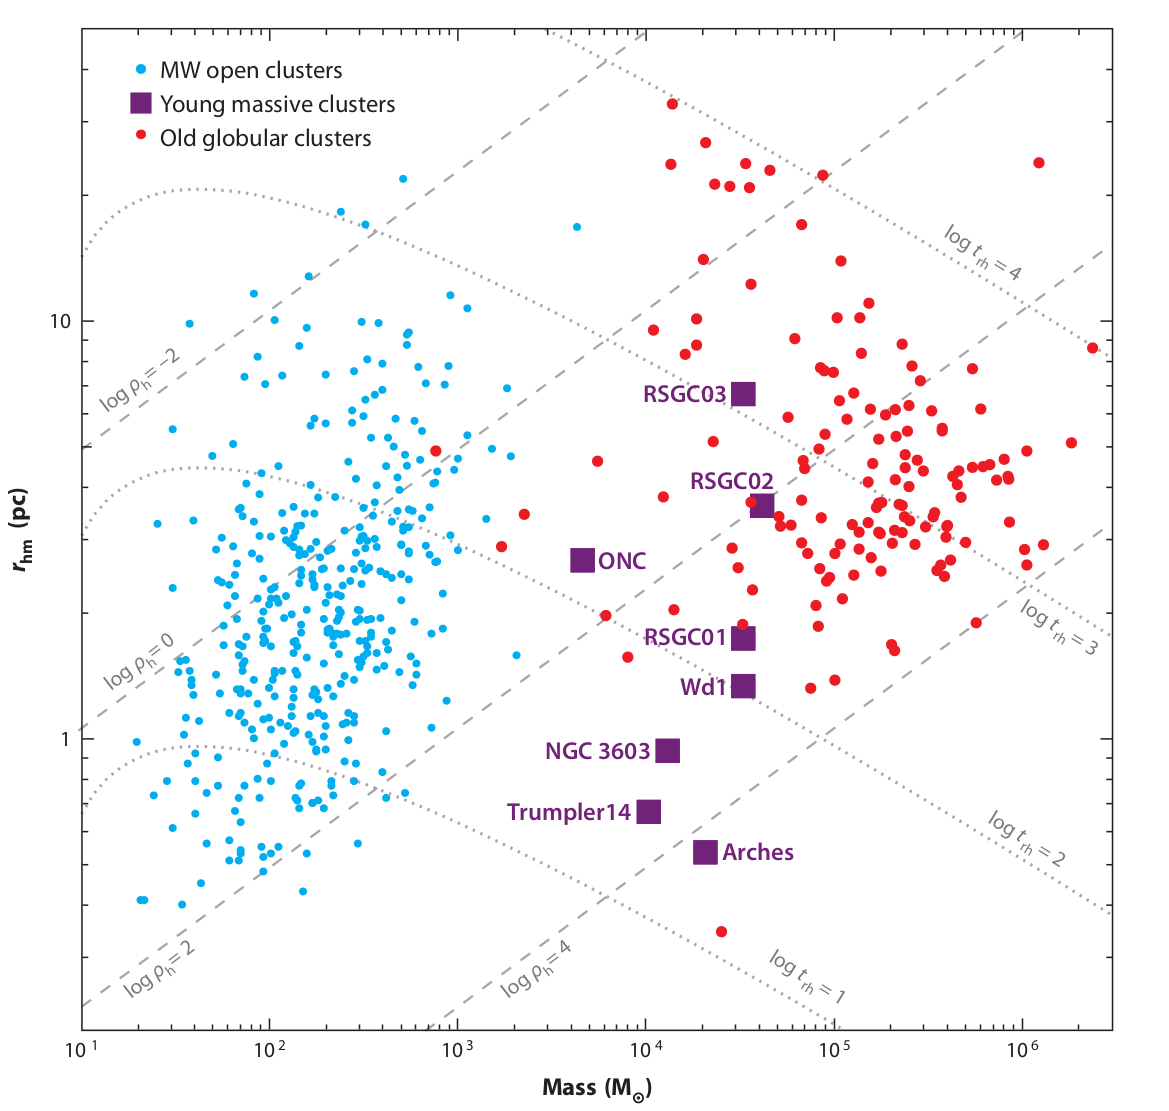
\includegraphics[width=0.62\linewidth]{Figures/0_MassRadiusClusters.png}
\caption{Radius-Mass Diagram for Milky Way clusters. Blue dots are open clusters, red dots Globular clusters and purple squares show Young Massive Clusters. Dashed lines show constant density within half-mass radius $\rho_h = 3M/8\pi r^3_{hm}$ and dotted lines show constant half-mass relaxation time. The plot was taken from the review \protect\cite{PortegiesZwart2010}.}
\label{Fig:0_SPZ}
\end{figure}

\item[\textbf{Embedded clusters}] are the youngest star clusters in the sky. Most of the stars, protostars and cores are still inside their primordial cloud, dust obscuring their optical light. The development of infrared astronomy unveiled the internal structure of these objects. Embedded clusters are young ($<$10Myr) and observed to be substructured \citep{Kuhn2015a}. Some have ongoing star formation, like NGC 1333, a very young embedded cluster with both proto-stars and stars, see \cite{Foster2015} and Fig~\ref{Fig:0_openglobular2.emb}.

\item[\textbf{Young Massive Clusters}], or \textbf{YMCs}, are considered to be globular cluster progenitors. The review by \cite{PortegiesZwart2010} provides a definition of YMCs: bound systems more massive than $10^4 \Mo$ and younger than 100 Myr. Only a handful of such systems are known in the milky way (see Fig~\ref{Fig:0_SPZ}). The most studied YMC of the galactic neighborhood is R136, with a mass $\sim 10^5 \Mo$ \citep{Andersen2009}, see Fig~\ref{Fig:0_openglobular2.emb}. It is located in the Tarentula nebula, the most active known star forming region in the local group, inside in the Large Magellanic Cloud \footnote{A dwarf irregular galaxy orbiting the milky way.}. YMCs are found in large number in intense star forming environment such as starburst galaxies and galaxy mergers like the Antenna galaxies \citep{Whitmore2010}.

\end{itemize}





"Most stars form in clusters" is a recurring statement in the field of stellar and cluster formation. Near Infra-Red (NIR) studies of star forming region yielded a star formation rate from embedded clusters of $\sim 3\cdot10^3~\Mo ~\textrm{Myr}^{-1}~ \textrm{kpc}^2$ \citep{Lada2003} while the same estimation for field stars in the milky way gives $\sim3-7\cdot10^3~\Mo~\textrm{Myr}^{-1}~\textrm{kpc}^2$ \citep{Miller1979}. Another clue at the clustered nature of star formation is that high-mass O stars are for the vast majority, clustered, see \cite{DeWit2005}. Due to their short life, O stars are often observed at the very location of their birth, or not very far. However, recent observations by, e.g,  \cite{Gutermuth2011} shows a spatially hierarchical star formation. The spherical, concentrated clusters we observe are then the outcome of a merging process from subclusters. 




%Due to their age, GCs are dynamically evolved. Introducing the relaxation time, defined in \cite{BT} by:
%\begin{equation}
%\label{Eq:0_relaxation}
%t_{relax} = 0.1 \frac{N}{logN} t_{cross} = 0.1 \frac{N}{logN} \frac{R_{hm}}{\sigma}
%\end{equation}
%
%with $t_{cross}$ the crossing time, defining the time a star takes to cross the system and $\sigma$ the internal velocity dispersion. The relaxation time is the time it takes for a system to erase its initial condition, perturbation per perturbation. GCs have a relaxation time of about a Gyr, they are relaxed systems. Various models have been put forward for the structure of GCs, the King \citep{King1966} and Plummer \citep{Plummer1911} models are the most widely used.


%\item NGC 2808 is reported to contain 1.4 $10^6~\Mo$ \citep{Boyles2011}. 
%
%Globular clusters had long been thought to have an homogeneous stellar population. Yet, a study by \cite{Piotto2007} showed NGC 2808 contained at least three different stellar sequences. Many other GCs has been shown to contain multiple populations. As this cannot be explained by the natural age spread arising from a continuous star formation at the birth clusters, such observations have far-reaching implication on their formation scenario. Several hypothesis are being explored, such as GCs being the outcome of mergers \citep{Pasquato2016} or a sequence of distinct star forming events \citep{Dantona2016}, with no consensus for now.


%\begin{itemize}
%
%\item 47 Tucanae (NGC 104) is one of the most massive known globular cluster in the Milky Way. It is estimated to contain about 1.5.$10^6~\Mo$ and to be 13 Gyr old\citep{Forbes2010}. Its core is extremely dense, as many GCs, with a central density up to $10^6 \Mo/\textrm{pc}^3$. Such a concentration of stars is a favorable environment for stellar collisions, which create what is called \textit{stellar exoticae}, stellar object not following the standard evolutionnary path, such as blue stragglers. Blue stragglers are stars too luminous and too massive compared to the age of the cluster, likely formed out of colliding stars. 47 Tuc exhibits a population of such objects, as well as others: Cataclysmic variables, X-ray binaries, etc. These are the direct consequence of the very dense environment of globular clusters such as 47 Tuc.
%
%\item Messier 12 (NGC 6218) is on the light end of the mass spectrum with 9.$10^4~\Mo$ \citep{Marks2010}. Such a low mass is however thought to be due to the cluster's dynamical history. Globular clusters have orbits around the galaxy, some more dangerous than others. For example Palomar 5 is currently disappearing after violent encounters with the galactic center. A study by \cite{DeMarchi2006} showed M12's orbit probably also passes close to the galactic center. Subjected to the strong tidal forces of the galactic bulge, M12 would have lost about 4/5 of its original mass. This scenario is backed by the mass function of M12. The mass function is the distribution of stellar masses, and its slope is thought to be more or less universal, though it appears unusually flat in M12. The tidal shock would have preferentially depleted low mass stars, as a process known as mass segregation tends to have massive stars sink at the center and low-mass stars overpopulate the outskirts of the system. 
%
%\item NGC 2808 is reported to contain 1.4 $10^6~\Mo$ \citep{Boyles2011}. NGC 2808, as all others GCs, had long been thought to have an homogeneous stellar population. Yet, a study by \cite{Piotto2007} showed NGC 2808 contained at least three different stellar sequences. As this cannot be explained by the natural age spread arising from a continuous star formation at the birth of the cluster, such observations have far-reaching implication on its formation scenario, and those of many GCs with multiple populations. Several hypothesis are being explored, such as GCs being the outcome of mergers \citep{Pasquato2016} or a sequence of distinct star forming events \citep{Dantona2016}, with no consensus for now.
%
%\end{itemize}

%
%\begin{figure}
%\label{Fig:0_GlobularClusters}
%\center
%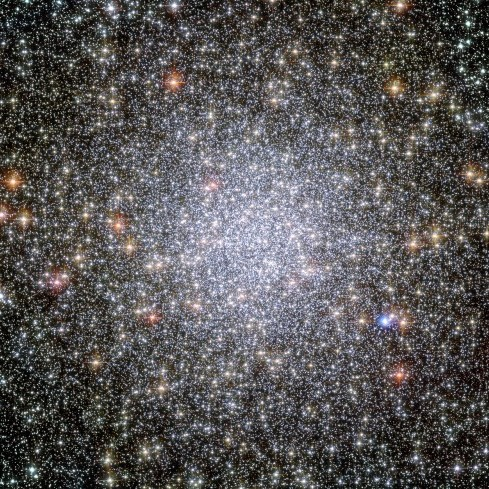
\includegraphics[width=0.3\linewidth]{Figures/0_47Tuc.jpg}
%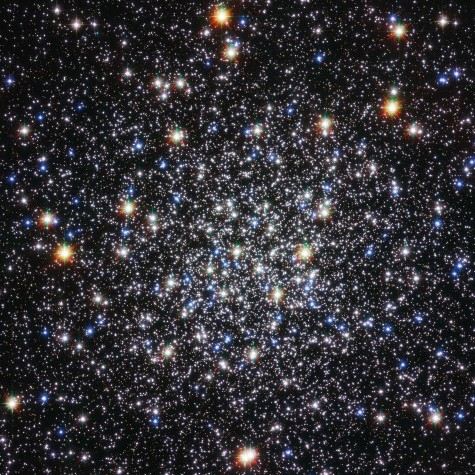
\includegraphics[width=0.3\linewidth]{Figures/0_M12.jpg}
%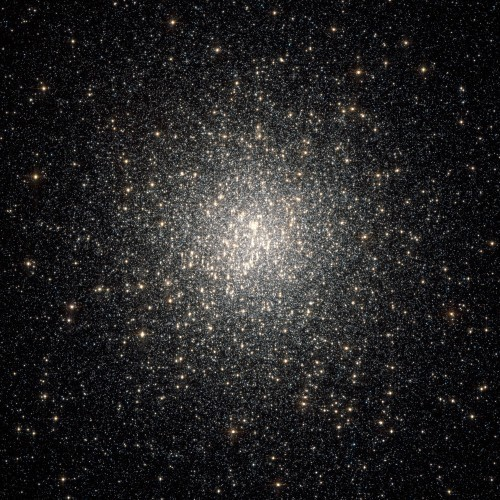
\includegraphics[width=0.3\linewidth]{Figures/0_NGC2808.jpg}
%\caption{From left to right: 47 Tucanae, Messier 12 and NGC 2808. Credits: ESA/Hubble. }
%\end{figure} 


\section{Some important dynamical concepts}

Before going into details about cluster formation and subsequent dynamical evolution, it is necessary to define some crucial dynamical concepts.

\subsection{Virial theorem}

A self-gravitating system is a system bound by its own gravity. This applies to a star, a molecular cloud, a star cluster or a galaxy. In all cases, gravity is set against a counteracting source of energy that prevents the total collapse of matter into a single point. This source can be pressure for stars and clouds, but for stellar systems such as clusters and galaxies, it is the agitation of its components, the kinetic energy of the stars. Other energy sources include magnetic pressure or tidal fields.

The exchange between the gravitational potential energy and the internal energy follows the virial theorem, written in the general form \citep{McKee2007,BT}:

\begin{equation}
\frac{1}{2} \frac{d^2 I}{dt^2} = 2 ( E_k - E_{k,s}) +  E_p + E_{tides} + E_m
\end{equation}
with $I$ the moment of inertia, $E_k$ the kinetic energy, $E_p$ the potential energy. $E_{k,s}$  a thermal pressure surface term, $E_{tides}$ the energy injected by a tidal field and $E_m$ the magnetic pressure. For a stationary system, $\frac{1}{2} \frac{d^2 I}{dt^2} = 0$, and in a purely gravitational system with N particles, there is no thermal or magnetic pressure. Finally, if we consider an isolated system, $E_{tides}=0$ and the virial theorem can be written in its more common form:

\begin{equation}
2 E_k + E_p = 0
\end{equation}

with :

\begin{equation}
 E_k = \sum_{i=1}^N  \frac{1}{2}m_i v_i^2 ~~~~\textrm{and}~~~~ E_p = - \sum_{i=1}^N \sum_{j>i}^N \frac{G m_i m_j}{\| \bold{r_i} - \bold{r_j}\| } .
\end{equation}

We define the virial parameter $Q$ as:
\begin{equation}
Q = - \frac{E_k}{E_p},
\end{equation}

$Q=0.5$ is a system in virial equilibrium. If the amplitude of the velocities is not sufficient to counteract the gravitational pull, $Q<0.5$, the system is said to be dynamically cold, or \textit{subvirial}. While if the stars are too close together compared to their velocities, $Q>0.5$, the system is hot and \textit{survirial}. If $Q>1$, the total energy is positive and the system is unbound. 


\subsection{Dynamical time-scales}
\label{Sub:0_time-scales}

Dynamical systems, like star clusters, tend to virial equilibrium. In such self-gravitating systems, it is useful to define a few dynamical time scales. The most simple one is the \textbf{crossing time}, defined as the time for a typical particle to cross the system. Following standard definitions \citep{Meylan1997,Fleck2006}, it is expressed as 

\begin{equation}
\label{Eq:0_tcr}
     \tc = \frac{2R_h}{\sigma} = \frac{2 R_h}{\sqrt{GM/R_g} } \, ,
\end{equation}
where $R_h$ is the half-mass radius, $\sigma$ the three-dimensional velocity dispersion, $M$ the mass of the system of gravitational radius $R_g$ given by $GM / R_g = \sigma^2$. 

Another crucial time-scale in stellar dynamics is the \textbf{relaxation time}, which can be defined as \citep{Heggie2003}:

\begin{equation} 
\label{Eq:0_trel}
\frac{\trel}{\tc} = \frac{0.138}{2} \left(\frac{R_h}{R_g}\right)^{1/2} \frac{N}{\ln 0.4 N}  
\end{equation}

In a self-gravitating system, stars have orbits. If N is large enough, the potential inside the system is smooth and stars have stationary orbits. The relaxation time is the time-scale at which the impact of numerous encounters a star endures is comparable to the motion of its initial orbit. In other words, the initial conditions of a system are dynamically erased by collisional evolution after a relaxation time.

In a relaxed cluster, the core is dense with a high velocity dispersion, whereas the outskirts, the halo, is less dense and stars are slower. The definition from equation (\ref{Eq:0_tcr}) and (\ref{Eq:0_trel}) imply the relaxation time changes with distance to the center. It is therefore useful to define a global time-scale for the whole system, the \textbf{half-mass relaxation time} defined by \cite{Heggie2003} as


\begin{equation}
\label{Eq:0_trhm}
t_{rh} \simeq   \frac{0.138}{\textrm{ln}(0.4 N)} \sqrt{ \frac{N}{G m}} R_h^\frac{3}{2}
\end{equation}

with $m$ the mass of a star and $R_h$ the half-mass radius. Let us compute two examples, taking G in appropriate units

\begin{equation}
G \simeq 4.48 \cdot 10^{-3}~~ \textrm{pc}^3 ~\textrm{Myr}^{-2} ~\Mo^{-1}.
\end{equation}

A cluster with 1000 stars of 0.5$\Mo$ and $R_{h} = 1$ pc has $t_{rh} = 13$ Myr, while a cluster with 10$^6$ stars of the same mass and a $R_{h} = 6$ pc has $t_{rh} = 3.1$ Gyr.


Equations (\ref{Eq:0_trel}) and (\ref{Eq:0_trhm}) assume identical stellar masses in the system. In a real cluster, stars have different masses, differently affected by collisional evolution. The most massive stars cause gravitational focusing and exchange energy with other stars at a higher rate. They lose their energy to lighter stars, progressively sinking at the center. \cite{Heggie2003} give an estimation of the segregation time-scale $t_{ms}(m_1)$ of a mass $m_1$,

\begin{equation}
\label{Eq:0_ms1}
t_{ms}(m_1) = \frac{m_1}{\langle m \rangle} t_{rh},
\end{equation} 
so a 30 $\Mo$ star in the previous 1000 star cluster will have a much shorter relaxation time of $\frac{0.5}{30} 13 = 0.21$ Myr = 210,000 years. A mass spread in a system speeds up considerably its collisional evolution.

A more general expression than (\ref{Eq:0_ms1}) can be obtained to quantify the global segregation time-scale. From \cite{Fleck2006}, the mass-segregation time-scale writes

\begin{equation}
\label{Eq:0_ms2} 
  \frac{\tms}{\trel} \equiv \frac{\pi}{3} \frac{\langle m_\star\rangle}{\max\{m_\star\}} \, \frac{\bar{\rho}_h}{\rho_g} \left( \frac{R_h}{R_g}\right)^{3/2} ,
\end{equation}
where $\bar{\rho}_h = M/2 /( 4\pi/3) R_h^3$ is the mean density within radius $R_h$, and $\rho_g$ the mean density inside a sphere of radius $R_g$.



\subsection{Static models}

It is useful to have a static reference model for a self-gravitating system at equilibrium. Considering a relaxed system with enough particles, one can use a statistical description to model its evolution, namely the "collisionless Boltzmann equation"

\begin{equation}
\frac{\partial f}{\partial t} + \bold{v} \cdot \nabla_r f - \nabla \Phi \cdot \nabla_v f = 0,
\end{equation}
with $f(\bold{r},\bold{v},t)$ the phase space distribution and $\Phi$ the gravitational potential. There are several solutions to this equations, these are "static" models for star clusters as they are considered in equilibrium. Of course, the collisional equation can never be fully neglected and these models are approximations. We present here two models: Plummer and King. Both have a constant density in the center, the core, but they differ by their general behaviours. 


\begin{figure}
\center
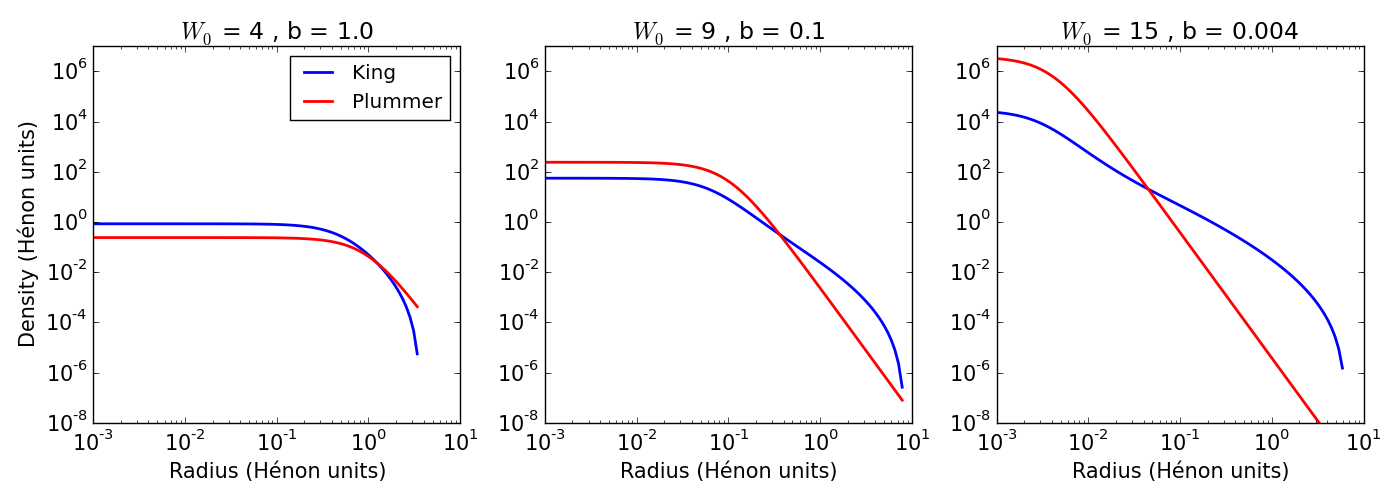
\includegraphics[width=0.95\linewidth]{Figures/0_kingplummer.png}
\caption{Comparison of King and Plummer models density as a function of radius, for similar core radiuses.}
\label{Fig:0_plummerking}
\end{figure}


The \textbf{Plummer model} is a simple model with a null potential at infinity. It is defined by its potential as a function of radius \citep{BT}:

\begin{equation}
\Phi(r) = - \frac{G M}{\sqrt{r^2 + b^2}}
\end{equation}

with $b$ the Plummer parameter, setting the depth of the central potential and the core radius. From this expression, one can derive the radial density distribution:

\begin{equation}
\label{Eq:0_plummerrho}
\rho(r) = \frac{3 M}{4 \pi b^3} \left( 1 + \frac{r^2}{b^2} \right) ^{- \frac{5}{2}}
\end{equation}

Equation (\ref{Eq:0_plummerrho}) makes the computational generation of a cluster straightforward, which is why the Plummer model has been widely used in numerical simulations of star clusters.
However, a Plummer model theoretically extends to infinity, and is not consistent with many globular cluster observations. Another, more complex, model has the observers on his side. The \textbf{King model} has been sucessfully used to fit light-profiles of globular clusters \citep{King1981}. It is defined as a distribution in energy:

\begin{equation}
  f_k(E)=\begin{cases}
    f_0 \left(e^{-2j^2E} - e^{-2j^2E_0}\right)  , & \text{if $E<E_0$}.\\
    0, & \text{otherwise}.
  \end{cases}
\end{equation}

with j a free parameter. The core radius can be tuned through a parameter $W_0 =2j^2(E_0 - E_c)$ with $E_c$ the rest energy at the center. 

The main difference with the Plummer model can be seen in Fig~\ref{Fig:0_plummerking}: for a given core radius, King's density decreases slower than Plummer, but does falls to zero at a given radius contrary to Plummer that continues to infinity.






\section{The origin of star clusters}

In this section, we describe the current understanding of star formation and its substructured spatial distribution in relation to that of the ISM. We then describe the dynamical evolution brought by this distribution and how it relates to the expulsion of the primordial gas by the young stars.


\subsection{From gas to stars}

The interstellar medium, or ISM, is made of dust and gas in various phases, densities and temperatures, ranging from a hot ionized medium ($T>10^5 $~K and $n < 0.01 ~\cm^{-3}$) to a cold neutral medium ($T<100$~K and $n > 10 ~\cm^{-3}$),  see \cite{Field1969}. Finally, in colder denser regions, $T\sim 10$~K and $n>30~\cm^{-3}$, the hydrogen takes molecular form H$_2$ in what is called molecular clouds. The dust contained in these regions makes them optically thick, obscuring background stars. These "holes in the sky", as William Herschel exclaimed upon the Dark Ophiucus Nebula\citep{Houghton1942}, come in different sizes, from the Bok globules to GMCs.
The interstellar dust absorbs the light in the visible and re-emits it in the infrared, thus the advent of infrared astronomy unveiled the interior of molecular clouds. In particular, recent observations with the Herschel Space Observatory showed a prevalence of filaments in clouds, see \cite{Andre2010} and Fig~\ref{Fig:0_horsehead}.

Star formation occurs in the higher density clumps or filaments inside the clouds. The origin of these overdensities has been the object of extensive theoretical development for 60 years. Turbulent motion was very early on designated as the main cause of overdensity. Turbulence is the transfer of energy from large scales to small scales, creating motions on small scales from a large energy driver. The well known Kolmogorov incompressible turbulence is hardly applicable to the ISM, as it is highly compressible \citep{Scalo1998}, instead, molecular clouds are subject to supersonic turbulence, or Burgers turbulence \citep{Frisch2001}. Nearby supernovas or tidal perturbation feed energy into the cloud, which is transferred through turbulence to smaller scales as supersonic internal motions, shocks forming overdense sheets. \cite{McKee2007} argue that filaments originate both from the intersection of such sheets and the primordial morphology of the cloud, as self-gravitating matter tends to condense as filaments \citep{Springel2005}.

\begin{figure}
\center
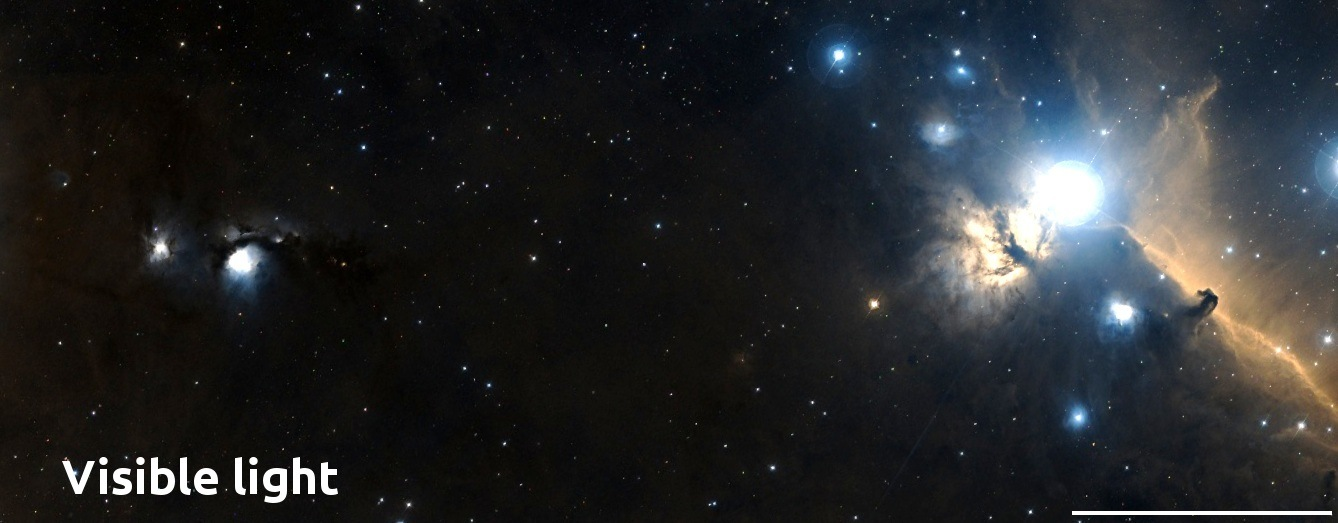
\includegraphics[width=0.95\linewidth]{Figures/0_horsehead_visible2}
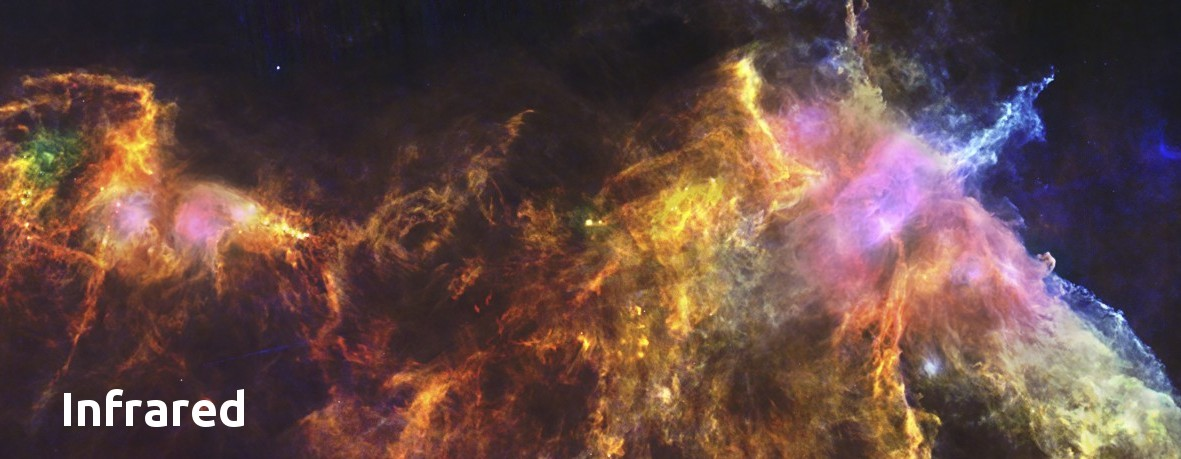
\includegraphics[width=0.95\linewidth]{Figures/0_horsehead_infrared}
\caption{Visible light  and infrared view of a part of the Orion star forming complex. Horshead nebula is visible on the right, as well as the very bright star Alnitak, part of the Orion belt. NGC 2071 and 2068 are visible on the left. Pink infrared coloring shows radiation from very bright young massive stars forming in the cloud. Colder filaments are visible all around. White bar on lower right of upper panel shows 1 parsec. \textit{Credits: Digitized Sky Survey; ESA/Herschel/PACS}. }
\label{Fig:0_horsehead}
\end{figure}

Individual condensates of matter called cores form in clumps and filaments, these are stellar seeds (Fig~\ref{Fig:0_proto_1}). They collapse when their self-gravity overcome their magnetic and thermal pressure and internal turbulence. When the central temperature increases and all molecular hydrogen has been dissociated, the collapse stops and the protostar is born (Fig~\ref{Fig:0_proto_2}). It starts accreting its gaseous envelope. Angular momentum from the original cloud shapes the envelope into a disk around the protostar, and magnetic activity starts creating jets (Fig~\ref{Fig:0_proto_3}). After about a Myr, accretion stops and the object becomes a Pre-Main Sequence (PMS) star (Fig~\ref{Fig:0_proto_4}). It slowly contracts, following the \cite{Hayashi1961} track, to finally reach 10$^6$K in its core and start fusing hydrogen into Helium. The  object enters the Main Sequence and begin its life as a "proper" star (Fig~\ref{Fig:0_proto_5}). See \cite{Larson1969} for a theoretical overview of the principles of collapse and protostellar formation. 

%The idealized picture of an hydrodynamical collapse relies on an estimation of the Jeans length $\lambda_\textrm{J}$, the maximum wavelength of a density perturbation in a uniform gas above which pressure cannot respond fast enough to avoid gravitational collapse. The corresponding Jeans mass M$_\textrm{J}$, of diameter $\lambda_\textrm{J}$ is the minimum mass of a cloud to collapse. These quantities are derived in \cite{BT} and are expressed
%
%\begin{align}
%\lambda_\textrm{J} & = \sqrt{\frac{\pi}{G \rho}} c_s \\
%	 & \simeq  0.2 \textrm{pc} \left( \frac{c_s}{0.2 ~ \textrm{km.s}^{-1}} \right) \left( \frac{n}{10^3 ~ \textrm{cm}^3} \right)^{-\frac{1}{2}}
%\end{align}
%
%\begin{align}
%M_\textrm{J} &=  \frac{4 \pi}{3} \rho  \lambda_\textrm{J} ^3 =    \frac{\pi}{6}  \frac{c_s^3}{G^\frac{3}{2}\rho^\frac{1}{2}} \\
% & \simeq  2.7 \Mo \left( \frac{c_s}{0.2 ~ \textrm{km.s}^{-1}} \right)^3 \left( \frac{n}{10^3 ~ \textrm{cm}^{-3}} \right)^{-\frac{1}{2}}
%\end{align}
%
%with $c_s$, $\rho$ and $n$ the local sound speed, density and number density. These are the typical values expected for a prestellar core with such sound speeds and number densities. It is reasonable to assume the gas remain isothermal for the first part of the collapse, as the center radiates away the thermal energy from the increased density. When density reaches $10^{10}$ cm$^{-3}$, the dust mixed in the protostellar material turns the core of the cloud optically thick, energy cannot be radiated away any more, temperature rises and collapse stops. Material continues to accumulate in the center, increasing the central density and temperature. When T reaches 2000K, molecular hydrogen starts to dissociate, absorbing energy. This allows a second collapse, stopped when all initial molecular hydrogen has been dissociated. The resulting core is called a protostar (Fig~\ref{Fig:0_proto_2}), its density profile is peaked in the center and reaches about $10^{21}$ cm$^{-3}$ and a temperature of 20,000K. The protostar has a mass of $\sim$ a thousandth of its future stellar mass, as most of it is acquired through accretion of the envelope. Angular momentum from the original cloud shapes the gaseous envelope into a disk around the protostar, and magnetic activity starts creating jets (Fig~\ref{Fig:0_proto_3}). This stage has been divided into several classes, based on the Spectral Energy Distributions (SED) emitted by the objects, as the emission shifts from far infrared to mid, then near-infrared as the envelope is accreted. See \cite{Evans2009} for an historical description of the SED classes and \cite{Larson1969} for a theoretical overview of the principles of collapse and protostellar formation. 



\begin{figure}
    \centering
    \begin{subfigure}[b]{0.19\textwidth}
        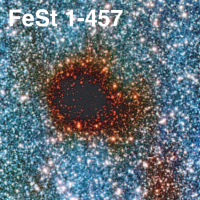
\includegraphics[width=\textwidth]{Figures/0_proto_1.jpg}
        \caption{  Starless core\\\centering (NIR)}
        \label{Fig:0_proto_1}
    \end{subfigure}
    \begin{subfigure}[b]{0.19\textwidth}
        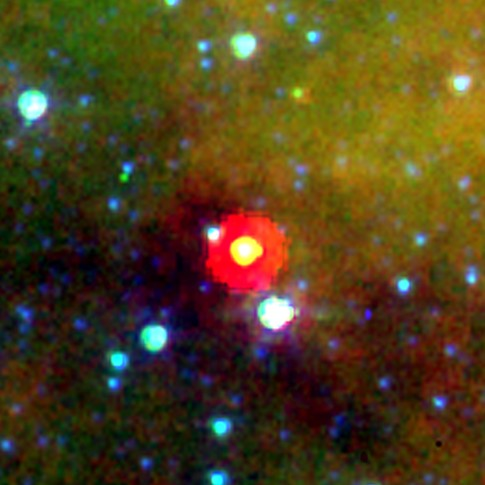
\includegraphics[width=\textwidth]{Figures/0_proto_2.jpg}
        \caption{Young protostar  \\ \centerline{ (IR)}}
        \label{Fig:0_proto_2}
    \end{subfigure}
        \begin{subfigure}[b]{0.19\textwidth}
        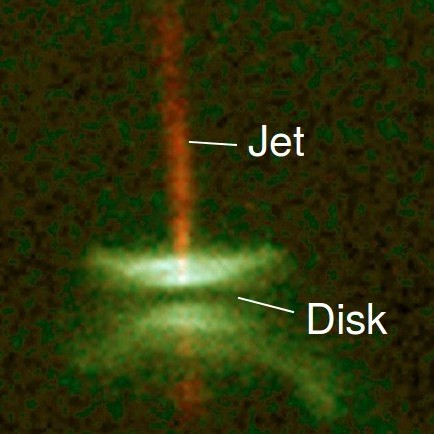
\includegraphics[width=\textwidth]{Figures/0_proto_3.jpg}
        \caption{Protostar \\\centering (IR,UV)}
        \label{Fig:0_proto_3}
    \end{subfigure}
        \begin{subfigure}[b]{0.19\textwidth}
        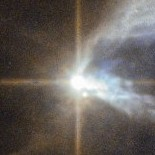
\includegraphics[width=\textwidth]{Figures/0_proto_4.jpg}
        \caption{Pre-MS star \\ \centering (visible)}
        \label{Fig:0_proto_4}
    \end{subfigure}  
        \begin{subfigure}[b]{0.19\textwidth}
        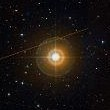
\includegraphics[width=\textwidth]{Figures/0_proto_5.jpg}
        \caption{MS star \\\centering (visible) }
        \label{Fig:0_proto_5}
    \end{subfigure}
     \caption{Stages of stellar birth. (a) is just cold molecular gas and contains no central source yet. (b) is more advanced, though hidden in visible light, its central protostar shines in infrared.The protostar in (c) is actively accreting its disk and produces jets. (d) is a pre main-sequence star, free from its envelope and surrounded by primordial gas. (e) is the mature stellar stage: the main sequence.\textit{Credits: \protect\cite{Kandori2005}; NASA/JPL-Caltech/Evans,N; Burrows,C/HST-NASA; ESA/Hubble \& NASA; DSS}}
     \label{Fig:0_protoevolution}
\end{figure}








\subsection{Substructure and early dynamical evolution}

These stars emerges from molecular clouds, which are observed to be heavily substructured (see e.g. \citealt{Cambresy1999}). This substructure can be seen as a fractal distribution \citep{Elmegreen1996} or a network of filaments \citep{Andre2010}, both consistent with compressible turbulence \citep{McKee2007}. Cores and protostars inherit this hierarchical structure as many observational studies of star forming regions, or substructured young clusters, show \citep{Schneider1979,Hartmann2002,Bressert2010}. See for example the distribution of Young Stellar Objects in the Carina Nebula on Fig~\ref{Fig:0_carina}. Examples of substructured young clusters include the Taurus Ariga region, $\rho$-Ophiucus and Aquila, details and other examples can be found in both volumes of \textit{The handbook of star forming region} \cite{Reipurth2008}.  

However, other young clusters do not display such fractal, clumpy or filamentary structure. Instead, they are smooth, centrally condensed systems. The most known example is the Orion Nebula Cluster, or ONC. Located in the heart of the Orion complex, the largest and most active star forming region in the solar neighborhood, the age of the ONC is estimated to a few Myr. \cite{Hillenbrand1998} found no clumps or filaments in the stellar distribution of the cluster, but a smooth distribution with a high density core formed by the Trapezium, a dense system of massive stars. This mass segregation, if not fully primordial, implies that some amount of dynamical evolution took place in the ONC since the formation of the stars. This dynamical evolution could have erased the initial substructures.

This is consistent with observations by \cite{Andre2007} who found clumps of prestellar objects to have a very low velocity dispersion in Ophiucus, meaning these clumps are more likely to merge and interact than diverge and disperse in the field.

These observations point at a rough picture of substructured stellar formation and early evolution: when the newly born stars emerges in clumps, if the background tidal field is weak and the star forming region sits well inside its Roche radius, the clumps then progressively merge and converge to the system barycentre to form a unique, relaxed  self-bound association over the course of a few crossing time. This picture is backed up to some extent by hydrodynamical simulations of fragmentation modes in the turbulent ISM \citep{Klessen2000,Bate2003,MacLow2004,Offner2009,Maschberger2010} and by recent observationnal clues that subclusters show dynamical traces of mergers \citep{Kuhn2015b}. 


\begin{figure}
\center
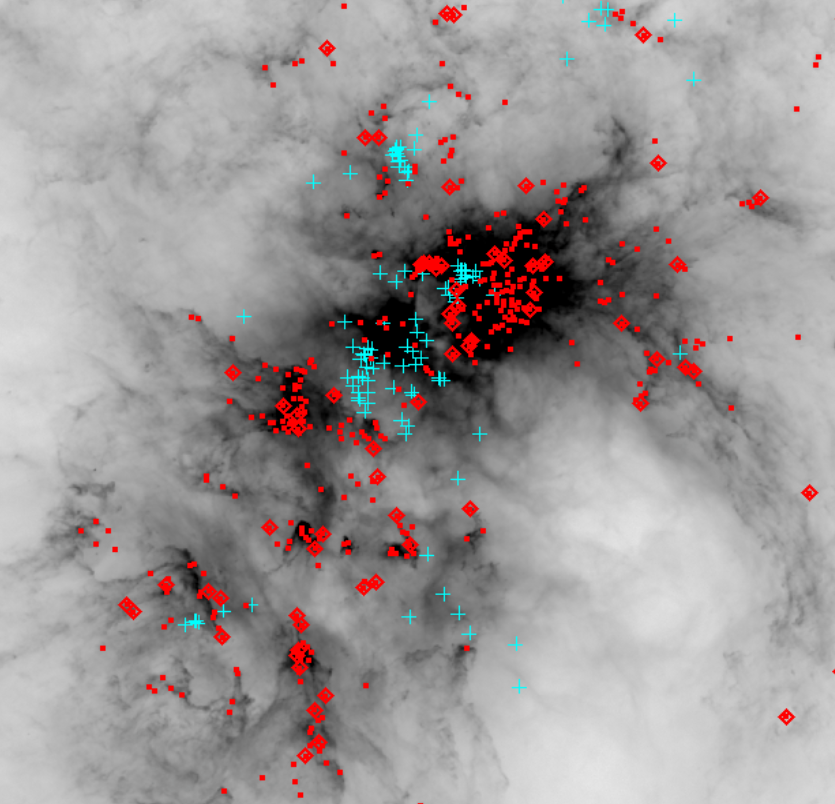
\includegraphics[width=0.7\linewidth]{Figures/0_carina}
\caption{Herschel IR 70µm observations of the Carina Nebula, with YSOs as red points and diamonds. Cyan crosses show OB stars. Both the gas and prestellar objects follow a substructured distribution. The figure was extracted from \cite{Gaczkowski2013}.}
\label{Fig:0_carina}
\end{figure}



%\begin{figure}
%\center
%    \centering
%    \begin{subfigure}[b]{0.48\textwidth}
%        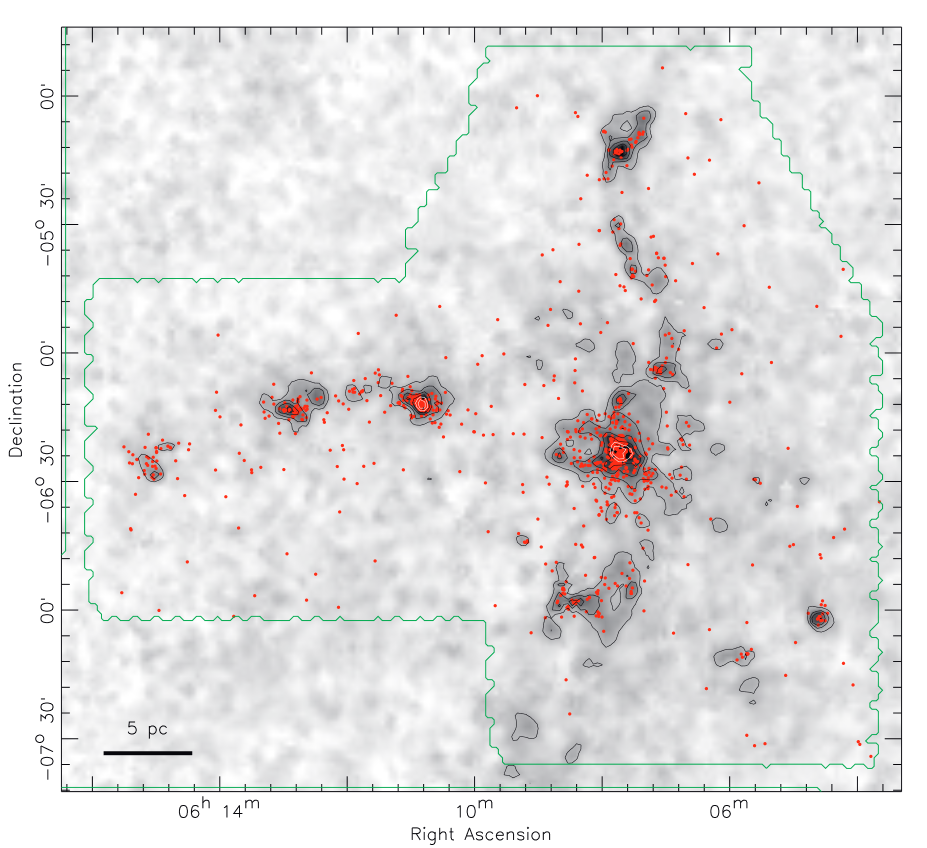
\includegraphics[width=\textwidth]{Figures/0_clumpsobserved.png}
%        \caption{Observed distribution of gas and protostars}
%        \label{Fig:0_clumps_obs}
%    \end{subfigure}
%    \begin{subfigure}[b]{0.48\textwidth}
%
%        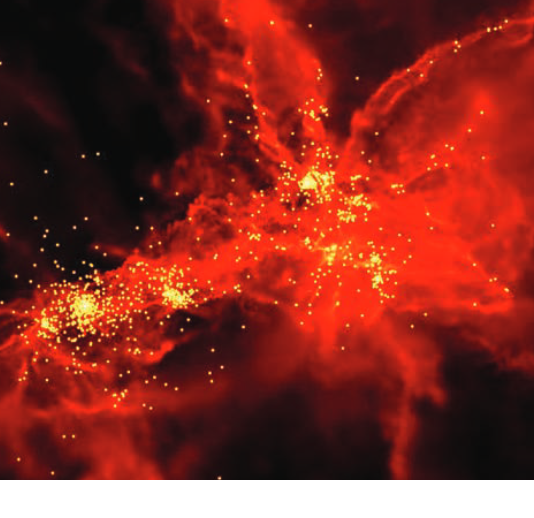
\includegraphics[width=0.9\textwidth]{Figures/0_clumpssimulated.png}
%        \caption{Hydrodynamical simulation}
%        \label{Fig:0_clumps_sim}
%    \end{subfigure}
%\caption{(a): observational data from the Monoceros R2 star forming region. Protostars are shown as red  points and gas density (traced through extinction) is shown in greyscale. The figure was extracted from \cite{Gutermuth2011}. (b): hydrodynamical simulation of a star forming region yellow points are star-like sink particles and red levels show gas density. The figure was extracted from \cite{Bonnell2011}.}
%\label{Fig:0_clumps}
%\end{figure}
%


\subsection{Star formation efficiency and infant mortality}

Though stars form in a hierarchical clumpy structure, star forming regions are vulnerable to gas expulsion and dispersion. 

\begin{figure}
\center
    \centering
    \begin{subfigure}[b]{0.48\textwidth}
        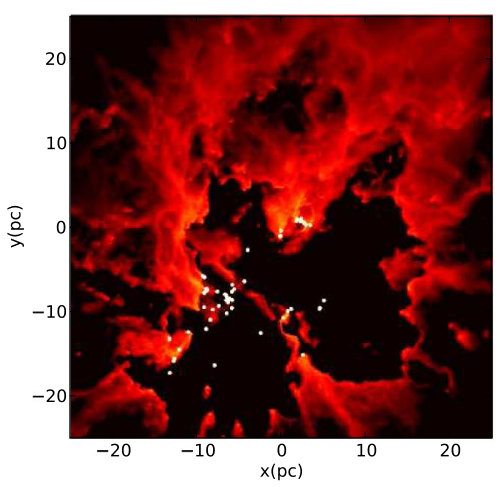
\includegraphics[width=0.9\textwidth]{Figures/0_ejectionwind.png}
        \caption{Simulation of gas expulsion}
        \label{Fig:0_ejection_1}
    \end{subfigure}
    \begin{subfigure}[b]{0.48\textwidth}

        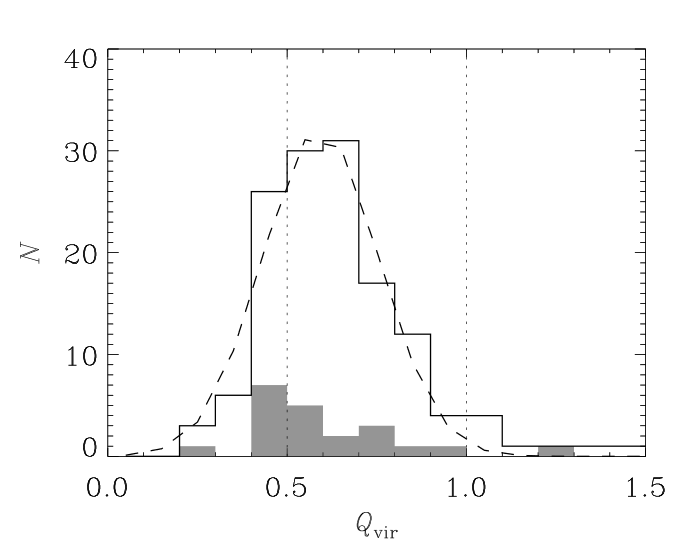
\includegraphics[width=\textwidth]{Figures/0_virializedclumps.png}
        \caption{Virial states of stellar clumps}
        \label{Fig:0_ejection_2}
    \end{subfigure}
\caption{(a): hydrodynamical simulation of wind-induced gas expulsion around a small cluster, the figure was extracted from \cite{Dale2013}. (b) virial parameter of stellar clumps in a star forming hydrodynamical simulation, ignoring the potential of the gas to predict their post-expulsion fate. The solid line is the cumulated distribution of clumps over all snapshots; the shaded histogram shows the final distribution. The figure was extracted from \cite{Kruijssen2012}.}
\label{Fig:0_clumps}
\end{figure}

In their seminal paper on embedded clusters, \cite{Lada2003} coined the term "infant mortality" for young star clusters. Comparing the populations of embedded clusters and older open clusters, the authors concluded clusters had a 90\% mortality rate before 10~Myr. This is explained by the traditionnal picture of gas expulsion in clusters: a portion of the gas in a molecular clouds forms a group of protostars, which quickly accrete their envelope, then start nuclear burning. This portion is expressed as the star formation efficiency
\begin{equation}
\epsilon = \frac{M_*}{M_* + M_{gas}},
\end{equation} 
with $M_{gas}$ the remaining gas after star formation. This gas is thought to be ejected from the young cluster through photo-ionization (the UV radiation from massive stars ionizes the neutral gas which heats up and expands), jets and outflows (young stars ejecting matter during accretion), winds (ejection of matter from stars surfaces at high speeds), and supernovae (shockwave from the explosive death of a massive star). The gas expulsion occurs on a crossing time-scale, see \cite{Krause2016}. Considering a young cluster in dynamical equilibrium, the loss of the mass of the gas on such a short time-scale can unbound the system, as the stars velocities are now too high for the new potential well. The young cluster then dissolves following the gas expulsion.
This picture is backed up by observations of young dissolving clusters \citep{Bastian2006} consistent with corresponding numerical models \citep{Goodwin2006}. Extensive analytical and numerical work have explored this process, e.g. \cite{Tutukov1978,Hills1980,Lada1984,Adams2000,Boily2003a,Boily2003b}, with an estimated minimum star formation efficiency of 30\% to remain bound after gas expulsion.
%
%However, the picture is more complicated than it seems. First, the efficiency of stellar feedback is a complex problem, winds, photionisation and supernovaes have various impacts depending on the size and morphology of the clouds; they also seem to influence each other, for an overview of the problem see the serie of papers from \cite{Dale2011,Dale2013} and references therein. Furthermore, recent hydrodynamical simulations such as \cite{Pelupessy2012} show the exact time-scale of gas removal has a crucial importance on the fate of the cluster, with a slow removal allowing survival with $\epsilon$ as low as 5\%.
%
%Finally, most of the previously mentionned simulations assumed a relaxed embedded stellar system. However, as mentionned in previous section, star formation is substructured. Dynamical evolution between clumps and subclusters occurs on time-scales comparable to gas expulsion, making the stellar spatial distribution of huge importance for survival, as shown by \cite{Farias2015}. Hydrodynamical simulations (e.g \citealt{Kruijssen2012}) even point at subclusters being primordially bound and resistant to gas expulsion: Fig~\ref{Fig:0_ejection_2} show the distribution of virial parameter $Q$ of stellar clumps in the simulation, ignoring the gas potential. The vast majority have $Q<1$ and are expected to stay bound after expulsion. This is likely due to localized high $\epsilon$. Though such observations are difficult, \cite{Kuhn2015b} found many stellar subclusters to be bound after gas expulsion.

However, the picture is more complicated than it seems. The interaction between types of stellar feedback, such as winds, photoionisation and supernovaes, is not well understood \citep{Dale2011,Dale2013}, and their exact time-scales can have a large influence on cluster survival \citep{Pelupessy2012}. Another serious issue with the classical picture of gas expulsion is that star formation is substructured and clusters undergo dynamical evolution while the gas is being evacuated, making survival heavily dependant on the clumpy structure, as shown by \cite{Farias2015}. Hydrodynamical simulations and recent observations show stellar clumps can be resistant to gas expulsion even before global dynamical relaxation \citep{Kruijssen2012,Kuhn2015b}, see Fig~\ref{Fig:0_ejection_2} which shows the distribution of virial parameter $Q$ of stellar clumps in a simulation, ignoring the gas potential. The vast majority have $Q<1$ and are expected to stay bound after expulsion.


Substructure and dynamical evolution have a prominent place in the issue of cluster survival. In this work, we study this phenomenon without a hydrodynamical treatment of the gas to isolate purely dynamical effects.



\section{Simulating star clusters evolution}

In this section, we describe the general characteristics of the hydrodynamical simulations invoked
earlier in this introduction. We emphasize their qualities and shortcomings, of which their limited system size. We then turn to alternative methods to numerically reproduce the early dynamical evolution of star clusters.

\subsection{Hydrodynamical simulations}

To model the formation of a star cluster from a core-less molecular cloud is no easy task. The model has to reproduce turbulence, core condensation, gravitational collapse, accretion, and for the most realistic ones, stellar feedback, magnetic effect and dust chemistry. Two numerical paths has been explored in the past: AMR and SPH.

Adaptative Mesh Refinement, AMR, is an Eulerian approach. The hydrodynamical equations (conservation of mass, momentum, the equation of state) are discretized and solved on a grid of cells following the finite volumes methods (see the RAMSES code, \citealt{Teyssier2002}). Smoothed Particle Hydrodynamics, SPH, is a Lagrangian approach: instead of looking at inputs and outputs of matter in a cell, the gas is subdivided in particles free to move in the system. They are attributed a density, temperature and pressure. This method is akin to N-body integration, and many SPH codes can work as purely gravitational integrators. Even if these codes can handle high density contrast, the collapse and formation of a protostar can still bring the numerical computation to a standstill. The usual workaround is the use of sink-particles: passed a given density threshold, several gas particles are merged into a single point-like object able to accrete any infalling matter. This works well though it suppresses any physical process below this accretion limit, usually a few to a hundred AU. \citep{Bate1997}.




\begin{figure}
\center
    \centering
    \begin{subfigure}[b]{0.48\textwidth}
    	\centering
        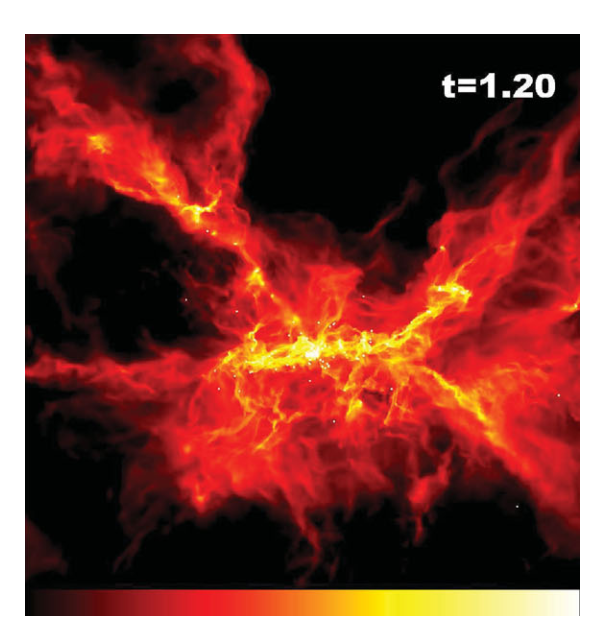
\includegraphics[width=0.9\textwidth]{Figures/0_bate2012.png}
        \caption{Observed distribution of gas and protostars}
        \label{Fig:0_bate2012}
    \end{subfigure}
    \begin{subfigure}[b]{0.48\textwidth}
        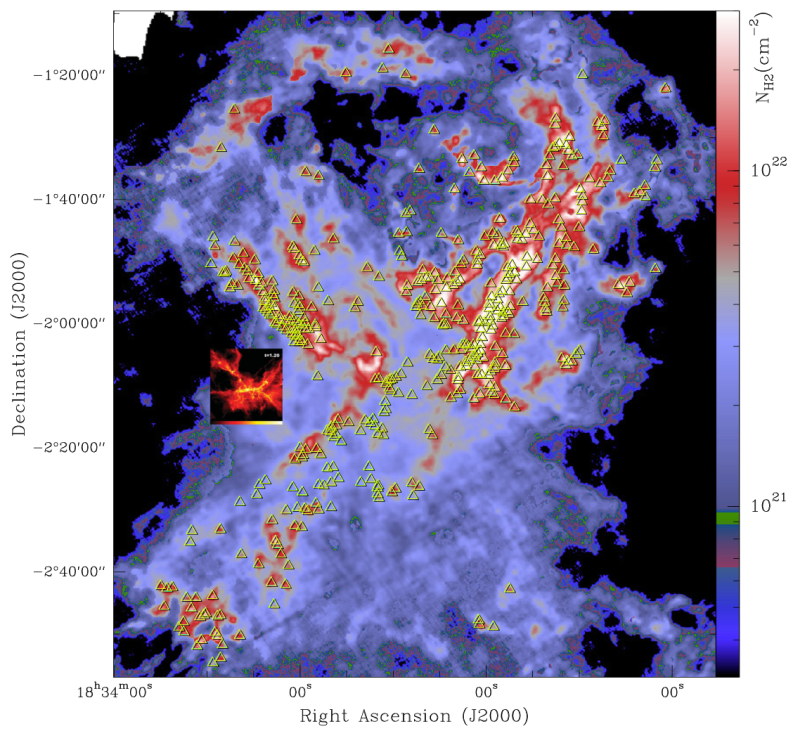
\includegraphics[width=\textwidth]{Figures/0_aquila_bate.png}
        \caption{Hydrodynamical simulation}
        \label{Fig:0_aquila_bate2012}
    \end{subfigure}
\caption{Comparison of star formation hydrodynamical simulation from \cite{Bate2012}  on (a) and Herschel infrared observations of the Aquila star forming complex, extracted from \cite{Konyves2010} on (b). Gas column density is shown as levels of red and yellow on the left and as levels of blue and red on the right. The simulation spans 0.6 parsecs while the observations, with the distance estimate from the authors, span 7 parsecs. We inserted the simulation into the observation to compare the scales.}
\label{Fig:0_clumps}
\end{figure}



The precision, size and complexity of cluster formation simulations have been steadily improving for 20 years (see \citealt{Turner1995,Klessen2000,Bate2003,Offner2009,Myers2014} and references). Nevertheless, no simulation to date include realistic cooling processes, radiative and wind feedback, magnetic fields and dust chemistry, all at the same time. All these are crucial to achieve precise and realistic simulation of the star formation process. Moreover, one of the most detailed star formation simulations to date, e.g \cite{Bate2012}, only form a few hundred stars in a volume spanning less than 1 pc and evolved them for less than 0.2~Myr with a simulation run time of several months. In fact, while looking at a typical star forming region, hydrodynamical simulations often reproduce a single fragment, see Fig~\ref{Fig:0_aquila_bate2012}.

However, good results are already being achieved, see the short review by \cite{Clarke2012}. Stellar properties and general structure agree with observations and interesting results are being obtained. \cite{Maschberger2011} and \cite{Moeckel2011} have noted that massive stars tend to sit at the heart of gas clumps in hydrodynamical simulations, some as the result of merger events with low-mass proto-stars. The hydrodynamical treatement allows the formation of gaseous disks around protostars that can influence the dynamics on small scales.

In summary, though hydrodynamical simulations are not yet fully realistic, they provide a good approximation of reality for small clusters and allow exploration of early dynamical processes. However, they cannot model the dynamical interactions between stellar sub-clusters and their consequences on a more massive final system.


\subsection{Artificial substructure}
\label{Sec:0_substructure}

There is a persistent difficulty to bridge over self-consistently from the star formation phase, to the equilibrium configuration of bound clusters. Hydrodynamical calculations of star forming regions evolve for  up to a few $10^5$ years, when a stable configuration would require several $10^6$ years at typical cluster densities of $10^4$ to $10^5$ stars per cubic parsec. A way to overcome this issue is to switch to purely gravitational N-body simulations once the stars formed and most of the gas has been either accreted or expulsed. It is computationally less expensive and allows for longer integration of larger systems.

It is then essential to obtain a good model of the stars phase-space distribution at the end of a hydrodynamical simulation. While King and Plummer model have a known distribution one can sample from, no such thing exist for the clumps and filamentary structure of the newborn stellar objects in star-forming regions. Several methods have been explored to solve this.



\begin{figure}
\center
    \centering
    \begin{subfigure}[b]{0.48\textwidth}
        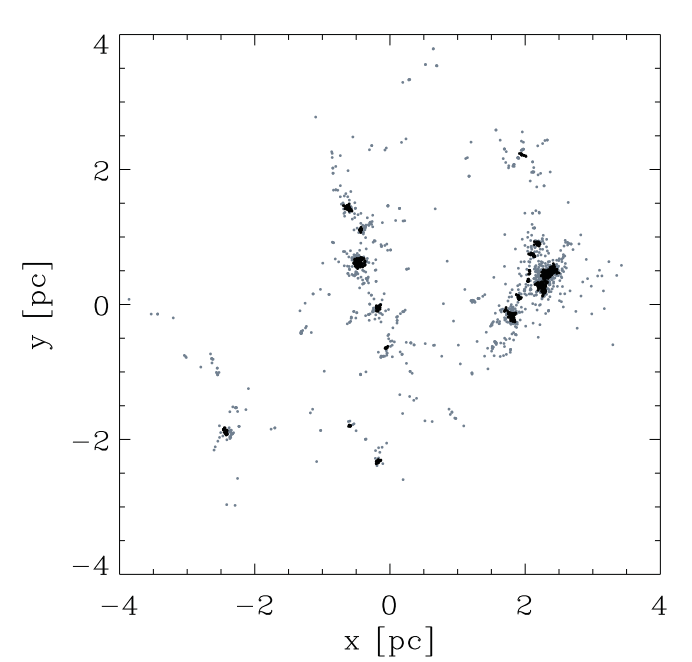
\includegraphics[width=\textwidth]{Figures/0_bonnell.png}
        \caption{Hydrodynamical output}
        \label{Fig:0_substructure_0}
    \end{subfigure}
    ~~
    \begin{subfigure}[b]{0.48\textwidth}
        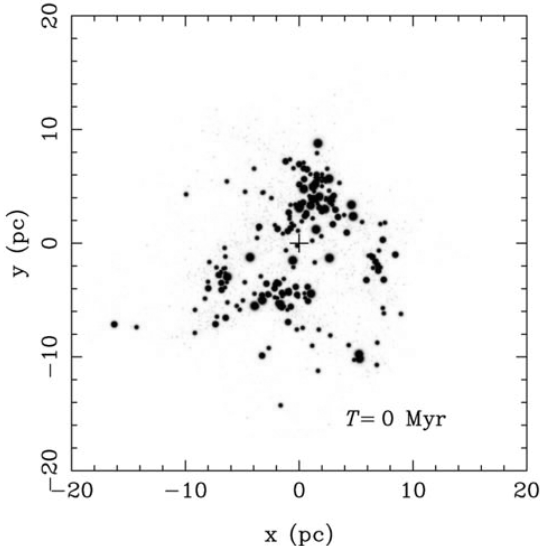
\includegraphics[width=0.93\textwidth]{Figures/0_fujii.png}
        \caption{Stellar spawning}
        \label{Fig:0_substructure_1}
    \end{subfigure}
    \\
    \begin{subfigure}[b]{0.48\textwidth}
        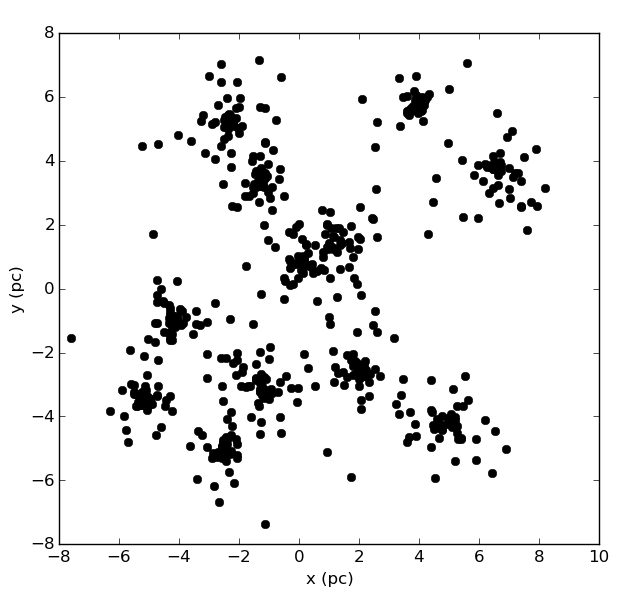
\includegraphics[width=0.95\textwidth]{Figures/0_plummers.png}
        \caption{Multiple Plummer}
        \label{Fig:0_substructure_2}
    \end{subfigure}
    \begin{subfigure}[b]{0.48\textwidth}
        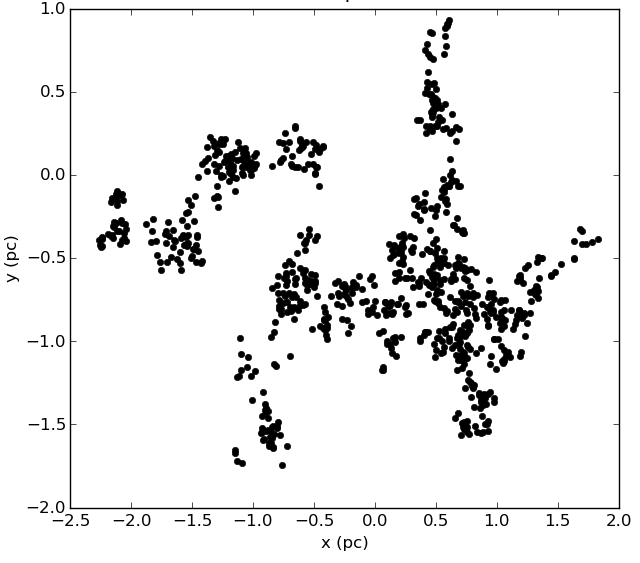
\includegraphics[width=\textwidth]{Figures/0_fractals.png}
        \caption{Fractal configuration}
        \label{Fig:0_substructure_3}
    \end{subfigure}
\caption{Representation of four methods to generate substructures. (a) is extracted from \cite{Kruijssen2012}, constructed with data from \cite{Bonnell2003}, (b) is extracted from \cite{Fujii2015}. (c) and (d) were generated for this work.}
\label{Fig:0_substructures}
\end{figure}

 
\begin{itemize}
\item[\textbf{Sink particle distribution}] is the most straightforward solution. \cite{Moeckel2010} took the distribution of sink particles formed in the hydrodynamical simulation by \cite{Bate2009} and directly converted it as a stellar distribution, preserving the masses, positions and velocities of the "stellar seeds". This is probably the best initial conditions for N-body simulations of young clusters that can be achieved, at the cost of speed, sampling and size. The initial hydrodynamical simulation took months to complete, making it hard to run it again and impossible to run it multiple times to obtain a good statistical sampling of the model. The size of the cluster achieved cannot exceeds a few 1000s stars given the current state of hydrodynamical simulations.

\item[\textbf{Stellar spawning from hydrodynamics}] is a variant of the previous method. \cite{Fujii2016} started from hydrodynamical simulations of massive molecular clouds and stopped the integration once the main structures had formed but before local gravitational collapse had set in. Stars were then spawned in space following the distribution of gas. This enables larger clusters and quicker initial conditions of structures. However, the velocity distribution of these new stars is artificial, as it can at best inherit the gas velocity, without including the impact of the early collisional evolution that occurs between protostars in the clumps.

\item[\textbf{Scattered Plummer spheres}] is an analytic answer to the substructure problem. \cite{McMillan2007} created a clumpy model for a young star cluster by spawning several Plummer spheres randomly in space. This is almost immediate and is a good approximation. The authors obtained interesting results on the inheritance of mass segregation during mergers. However, the Plummer profile places a constraint on the clumps internal dynamics which bias the dynamical evolution. 

\item[\textbf{Fractal models}] were introduced by \cite{Goodwin2004} and has been used in numerous studies ever since, e.g. \cite{Allison2009b,Kouwenhoven2010,Parker2016}. The idea is to grow a 3D pseudo-fractal tree with probabilistic branching, up to a given level, turning the final leaves into stars. The method is fast and the result is spatially realistic, fitting the observation that finds a fractal structure in the molecular clouds and star forming regions. However, the velocity distribution is artificial, drawn from successive gaussians at each levels. The clumps will relax when integration starts, shaking the whole system right off the bat.

\end{itemize}

It seems the generation of substructure has to balance realism and computational cost. The most realistic method is too costly, and most of the quicker alternatives are disconnected from the dynamical effect arising from the collisional effects young stars undergo inside a clumpy configuration. There is a need for an computationally efficient method to produce dynamically consistent initial conditions to model young star clusters and study their evolution, which is what we introduce in the next chapter.







